\documentclass{article}
\usepackage{graphicx}
\usepackage{amssymb,amsmath}
\usepackage{fancyhdr}
\pagestyle{fancyplain}
\rhead{Prepared by Adam Beardsley on \today}

\begin{document}

\section{Weights and variance of gridded visibilities}
We start with the rms of a visibility,
\begin{equation}\label{eq:vis_rms}
\sigma_v = \frac{2 k_B T_{sys}}{A_e \sqrt{d\!f \tau}}
\end{equation}
where $k_B$ is Boltzmann's constant, $T_{sys}$ is the system temperature, $A_e$ is the effective collecting area, $df$ is the frequency channel width, and $\tau$ is the single snapshot observation time.  We can easily plug in true observational parameters to give us the rms for individual visibilities.

\begin{equation}
\sigma_v = 2761.3006 \left(\frac{T_{sys}}{\text{K}}\right) \left(\frac{\text{m}^2}{A_e}\right) \left(\frac{\text{Hz}}{df}\right)^{1/2} \left(\frac{\text{sec}}{\tau}\right)^{1/2} \text{Jy}
\end{equation}
For example, if we have $T_{sys} = 440$ K, $A_e = 16$ m$^2$, $df = 40$ kHz, and $\tau = 5$ seconds, I get $\sigma_v \approx 169.8$ Jy.

Ian uses the model beam to grid the data (or the weights) into a regular $uv$ grid. As an example, let's look at a simplified case of two overlapping visibilities, and consider the gridded value and variance of a pixel in the overlapping region.
\begin{figure}[h!]
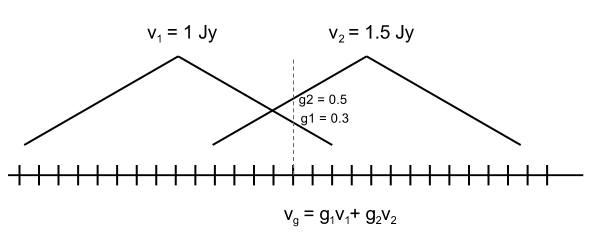
\includegraphics[width=\columnwidth]{vis_grid.png}
\caption{Gridding two visibilities}
\end{figure}

Each visibility ($v_1$ and $v_2$)is multiplied by the beam value at the pixel in question ($g_1$ and $g_2$) and added to produce the gridded visibility.
\begin{equation}
v_g = g_1 v_1 + g_2 v_2
\end{equation}
The variance on $v_g$ can easily be calculated using error propagation.
\begin{equation}\label{eq:grid_var}
\sigma_g = \sqrt{\left(g_1\sigma_1\right)^2 + \left(g_2 \sigma_2\right)^2} \approx \sigma_v \sqrt{g_1^2 + g_2^2}
\end{equation}
In the case that our antennas are identical, all the values in Eq. \ref{eq:vis_rms} are identical, so we can replace $\sigma_1$ and $\sigma_2$ with a common $\sigma_v$.

\vspace{.2cm}
[Adding snapshots in healpix\ldots need to figure this out\ldots]
\vspace{.2cm}

Ignoring the healpix business for now, we want to know what happens to our noise when we divide by the weights in $(u,v,f)$ space. The ``weights" we use are the sum of beam models in each pixel. In our simple example,
\begin{equation}
w_g = g_1 + g_2.
\end{equation}
This weight is an accurate description of how well we sampled each pixel on the $uv$ plane. Our best estimate of the apparent sky is then
\begin{equation}
\hat{v} = \frac{v_g}{w_g} = \frac{g_1v_1+g_2v_2}{g_1+g_2}.
\end{equation}

Again we can simply propagate error.
\begin{equation}
\sigma_{\hat{v}} = \frac{\sigma_g}{w_g} = \sigma_v \frac{\sqrt{g_1^2 + g_2^2}}{g_1 + g_2}
\end{equation}

From here we can form our covariance matrix and propagate through the frequency Fourier transform and square to power spectrum as Bryna has been doing.

{\bf Conclusion:} \, To me it seems like we need both the weights cube ($g_1 + g_2$ in the example above) as well as a cube where the beams were squared before the gridding ($g_1^2 + g_2^2$) in order to propagate the rms correctly.

\section{Covariance between grid points}
Because the same data is being gridded to multiple grid points, this gridded data is highly covariant. Here I will quantize this covariance.

Consider two grid points, indexed with $i$ and $j$, with $n$ visibilities contributing. In general the visibilities contributing to both grid points do not need to be identical (we are interested in cases where there is some overlap), but let $n$ represent the union of the two sets of visibilities. Then we have the gridded visibilities,
\begin{subequations} \label{eq:two_grids}
\begin{align} 
v_i &= \sum_n g_{n,i} v_n  \\
v_j &= \sum_n g_{n,j} v_n 
\end{align}
\end{subequations}
We wish to calculate the covariance.
\begin{equation}
C_{ij} = \left<(v_i-\bar{v}_i)(v_j-\bar{v}_j)^*\right>
\end{equation}
Angled brackets ($<...>$) represent an expectation value, and a bar is shorthand for the same. We can simplify this equation slightly before proceeding.
\begin{subequations}
\begin{align}
C_{ij} &= \left<v_iv_j^* - v_i\bar{v}_j^* - \bar{v}_iv_j^* + \bar{v}_i\bar{v}_j^*\right> \\
&= \left<v_iv_j^*\right> - \bar{v}_i\bar{v}_j^* - \bar{v}_i\bar{v}_j^* + \bar{v}_i\bar{v}_j^* \\
& = \left<v_iv_j^*\right> - \bar{v}_i\bar{v}_j^*
\end{align}
\end{subequations}

Now we plug in Eq. \ref{eq:two_grids}, and group terms appropriately.
\begin{subequations}
\begin{align}
C_{ij} &= \left<\sum_n g_{n,i}v_n \sum_m g_{m,j}^* v_m^* \right> - \sum_n g_{n,i}\bar{v}_n \sum_m g_{m,j}^* \bar{v}_m^* \\
&= \sum_n\sum_m\left(g_{n,i}g_{m,j}^* \left<v_n v_m^*\right> - g_{n,i}g_{m,j}^*\bar{v}_n\bar{v}_m^*   \right) \\
&= \sum_n\sum_m g_{n,i}g_{m,j}^* C_{nm}
\end{align}
\end{subequations}

We have now expressed our gridded covariance matrix in terms of the raw visibility covariance matrix. Thus far we have made no assumptions about the covariance of the visibilities, however, in order to simplify further I will assume that this covariance matrix is diagonal and all visibilities have the same variance (as we assumed above). Then we have the result,
\begin{equation}
C_{ij} =  \sigma_v^2 \sum_n g_{n,i}g_{n,j}^*.
\end{equation}
Now the sum over $n$ can be restricted to the intersection of visibilities that contribute to \emph{both} grid points. It is nice to see that in the case $i=j$, this result conforms to Eq. \ref{eq:grid_var}. Additionally, this is exactly the Holographic Mapping function used in FHD, which Ian already computes for every snapshot.

{\bf Conclusion:} The covariance matrix between grid points for a single snapshot is given simply by the Holographic Mapping function used in FHD. In principle we should be able to transform this function to the image space, add in healpix, and transform back in the same way we treat the data. The difficulty is the size of this matrix. It is sparse, which should help greatly in the transformation to image space, but it is not sparse there, and the transform back may be difficult. In addition, this adds to the work needed for the Fourier transform over frequency when calculating power spectra.

\section{Error propagation to power spectrum}

In the next steps we wish to arrive at a power spectrum measurement, using two interleaved data cubes along with their variances. I will assume we performed the frequency Fourier transform on the data and propagated the covariance cubes by applying the Fourier transform matrix on both sides. In this space, we have cubes $a_1(u,v,\eta)$ and $a_2(u,v,\eta)$ where 1 and 2 correspond to the two interleaved cubes. We also have $b_1$ and $b_2$ for the orthogonal mode (e.g. sine and cosine), but they are separated in most of the math, so I will focus on $a$'s for now.

The first thing we need to do is add and subtract the two cubes, accounting for the weights. From here on out, I will assume the ``weights" are the inverse of the variance, rather than the gridded constants from the previous section.
\begin{equation}
a_{sum} = \frac{w_{a1}a_1 +w_{a2} a_2}{w_{a1}+w_{a2}} ; \; \; \;
a_{sub} = \frac{w_{a1}a_1 -w_{a2} a_2}{w_{a1}+w_{a2}} 
\end{equation}
The variance of the results are
\begin{equation}
\sigma^2_{sum} = \sigma^2_{sub} = \frac{1}{w_{a1} + w_{a2}}.
\end{equation}
Because all we have done thus far is scale by weights and add, I believe we can perform this step in the $(u,v,f)$ space due to the linearity of the Fourier transform. This should allow us to avoid translating two weights cubes to $(u,v,\eta)$ space.

The next step is to perform a magnitude squared on both $a_{sum}$ and $a_{sub}$. The math is a little messy, so I will demonstrate it for an arbitrary complex number drawn from a symmetric gaussian distribution. We start with a probability distribution function for a number $c$.
\begin{equation}
\mathrm{Pr}(c) = \frac{1}{\pi \sigma^2} e^{-\left|c-\mu\right|^2/\sigma^2}
\end{equation}
Here $\mu$ is the mean complex value of the distribution, and $\sigma$ is the standard deviation of the \emph{complex number} $c$. It is important to distinguish this $\sigma$ from the standard deviation of the real and imaginary parts separately (which would be a factor of $\sqrt{2}$ smaller). Also note that the visibility rms given at the beginning of the last section is actually the real/imaginary version. So things aren't exactly perfect from here...

Next we find the pdf of $|c|$ which is found by integrating a ring of constant magnitude,
\begin{equation}
\mathrm{Pr}(|c|) = \int_0^{2\pi}d\phi \mathrm{Pr}(c)|c| = \frac{2 |c|}{\sigma^2} e^{-(|c|^2+|\mu|^2)/\sigma^2} I_0(\frac{2|c||\mu|}{\sigma^2})
\end{equation}
where $I_0$ is the $0^{\mathrm{th}}$ modified Bessel function. A change of variables takes us to the pdf for $|c|^2$.
\begin{equation}
\mathrm{Pr}(|c|^2) = \frac{d |c|}{d |c|^2} \mathrm{Pr}(|c|) = \frac{1}{\sigma^2} e^{-(|c|^2+|\mu|^2)/\sigma^2} I_0(\frac{2|c||\mu|}{\sigma^2})
\end{equation}

The stats we care most about here are the expectation value of $|c|^2$ and the variance of $|c|^2$. They are
\begin{subequations}
\begin{align}
\left< |c|^2 \right> & = |\mu|^2 + \sigma^2\\
\mathrm{var}(|c|^2) & = \sigma^2\left(2 |\mu|^2 + \sigma^2\right).
\end{align}
\end{subequations}

Back to the sum and difference cubes, we can now determine the expected values and variances of the magnitudes squared (taking $S$ to be the signal, and $\sigma^2$ is the inverse of the respective weight).
\begin{subequations}
\begin{align}
\left<\left|a_1+a_2\right|^2\right> & = |S|^2 + \sigma_{sum}^2 \\
\left<\left|a_1-a_2\right|^2\right> & = \sigma_{sub}^2
\end{align}
\end{subequations}
\begin{subequations}
\begin{align}
\mathrm{var}\left(\left|a_1+a_2\right|^2\right) & = \sigma_{sum}^2 \left(2 |S|^2 + \sigma_{sum}^2\right) \\
\mathrm{var}\left(\left|a_1-a_2\right|^2\right) & = \sigma_{sub}^4
\end{align}
\end{subequations}

We are almost there. Because our sum term has noise in its expected value, we must subtract the pure noise term to arrive at a best estimate of the signal.
\begin{equation}
\left|\hat{S}_a\right|^2 = \left|a_1+a_2\right|^2 - \left|a_1-a_2\right|^2
\end{equation}
Note that even though the two terms can have very different variances, this should \emph{not} be a weighted sum, or the noise would not subtract properly. The variance is
\begin{equation}
\sigma^2_{S,a} = \mathrm{var}\left(\left|a_1+a_2\right|^2\right) + \mathrm{var}\left(\left|a_1-a_2\right|^2\right) = 2 \sigma_{sum}^2\left(|S|^2 + \sigma_{sum}^2\right)
\end{equation}
where I have used the fact that $\sigma_{sum}=\sigma_{sub}$ to simplify slightly. At first look I thought these terms would be covariant and the error propagation would not be so easy. However, simple simulations have shown that the covariant terms are negligible. I have not fully understood this, but I think it has to do with the particular linear combinations being independent (similar to changing bases in vector space).


Finally we can include the $b$ terms to help our estimate slightly. 
\begin{equation}
\left|\hat{S}\right|^2 = \frac{w_{S,a}\left|\hat{S}_a\right|^2 + w_{S,b}\left|\hat{S}_b\right|^2}{w_{S,a}+w_{S,b}}
\end{equation}
With a variance on our final estimate being
\begin{equation}
\sigma^2_S = \frac{1}{w_{S,a}+w_{S,b}}.
\end{equation}

\section{PDF after averaging bins}

In this section I will describe the probability distribution function when we square complex numbers, then average bin (rings for 2D PS, shells for 1D PS). As in the last section, I will treat the two orthogonal modes in a $k$ bin separately (e.g. sines and cosines). They are combined in the averaging step with all the other modes in the bin.

We start with the PDF of a symmetric complex gaussian distributed number. Some of this is repeated from above, but I wish to put everything together. To conform notation to what Bryna uses in her code, $\sigma$ will now represent the uncertainty on the real and imaginary parts individually. I will also drop the mean value because we are currently particularly interested in the noise cubes.
\begin{equation}
\mathrm{Pr}(c) = \frac{1}{2\pi \sigma^2}e^{-|c|^2/2\sigma^2}
\end{equation}

Taking magnitude squared of $c$ gives us an exponential distribution with parameter $\lambda=1/2\sigma^2$.
\begin{equation}
\mathrm{Pr}(|c|^2) = \frac{1}{2\sigma^2}e^{-|c|^2/2\sigma^2}
\end{equation}
The expectation value and variance of this distribution are $1/\lambda = 2\sigma^2$ and $1/\lambda^2 = 4\sigma^4$ respectively.

The next step is to perform a weighted average in either rings or spherical shells. We assign the above distribution for each voxel $i$ and weight by the inverse variance to sum. Here we include the sine and cosine modes in the sum.
\begin{equation}
\overline{|c|^2} = \frac{\sum\lambda_i^2 |c_i|^2}{\sum \lambda_i^2}
\end{equation}
The expectation value and variance of the weighted sum are given by
\begin{subequations}
\begin{align}
\left<\overline{|c|^2}\right> & = \frac{\sum\lambda_i^2 \left<|c_i|\right>}{\sum \lambda_i^2} = \frac{\sum\lambda_i}{\sum \lambda_i^2} \\
\mathrm{var}(\overline{|c|^2})& = \frac{1}{\sum \lambda_i^2}.
\end{align}
\end{subequations}

The sum of exponentially distributed numbers with equal parameters yields an Erlang distributed number. The weighted sum does not exactly yield an Erlang distribution, but if the weights are reasonably uniform (within an order of magnitude of one another), we can well approximate the resulting distribution as Erlang with effective parameters. The PDF of an Erlang is given by
\begin{equation}\label{eq:erlang}
\mathrm{Pr}(z) = \frac{z^{n-1} e^{-z/\beta}}{\beta^n \Gamma(n)}
\end{equation}
where $n$ would be the number of voxels that went into the average if all weights were the same, and $\beta$ would be $1/\lambda$. Because our weights are not all the same some voxels contribute more than others, which leads to an effective number that went into the average less than the true number, and a variance more heavily weighted by the small variance voxels. We can solve for the effective parameters by writing down the mean and variance of this distribution, and setting them equal to those for our weighted average.
\begin{subequations}
\begin{align}
\left<z \right> & = n_{\mathrm{eff}} \beta_{\mathrm{eff}} = \frac{\sum\lambda_i}{\sum \lambda_i^2} \\
\mathrm{var}(z) & = n_{\mathrm{eff}} \beta_{\mathrm{eff}}^2 = \frac{1}{\sum \lambda_i^2}
\end{align}
\end{subequations}
Solving\ldots
\begin{subequations}\label{eq:erlang_params}
\begin{align}
n_{\mathrm{eff}} & = \frac{\left(\sum\lambda_i\right)^2}{\sum \lambda_i^2} \\
\beta_{\mathrm{eff}} & = \frac{1}{\sum\lambda_i}
\end{align}
\end{subequations}

We can test this parameterized fit with some simulated data. In Figure \ref{fig:erlang} we plot a histogram of simulated data obtained from squaring and averaging complex random numbers (ie. starting at the beginning of this section). 

The fit accurately predicts the shape of the distribution for a few voxels as well as for many. Where the fit breaks down is when the weights that go into the average are allowed to vary significantly. In the figure titles, the quantity `sigma SNR' refers to the average sigma divided by the standard deviation of the sigmas that went into the original simulation. As this number decreases, the predicted distribution (red line) deviates from the simulated data. In particular, we see int he last plot, when the sigma SNR is about 3 that the predicted distribution is not as peaked as the simulation.

More investigation is needed to determine if the voxels going into our averages will satisfy the large sigma SNR condition. However, this method can be tentatively used to predict the noise power and uncertainty in EoR data.

\begin{figure}
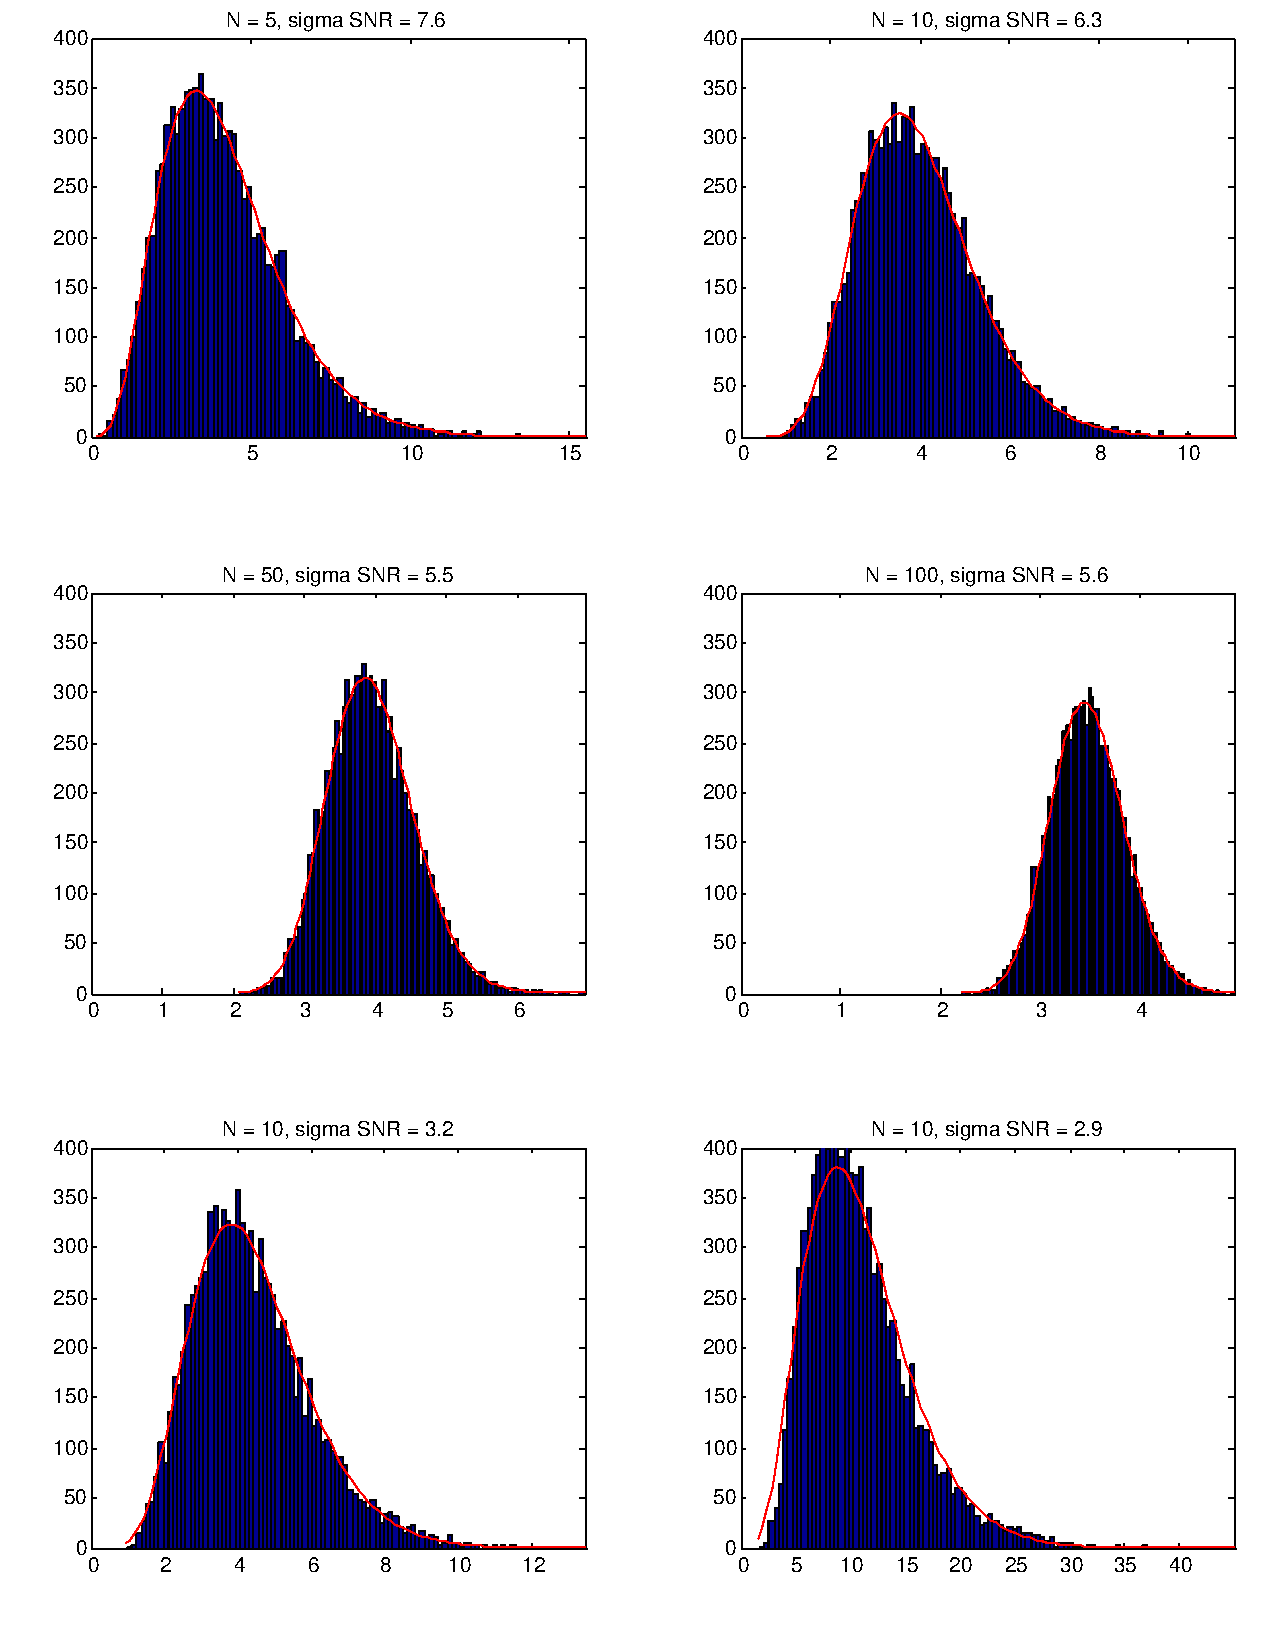
\includegraphics[width=\columnwidth]{erlang.pdf}
\caption{Simulated noise data against fit Erlang distributions}
\label{fig:erlang}
\end{figure}


\end{document}